% !TEX root =  main.tex

\chapter{Virtualized hosting platforms}
\label{ch: reconfiguration}

Over the last 20 years, the design of platforms dedicated to the execution of parallel and distributed applications has evolve from monolithic supercomputers to a flexible aggregation of interconnected servers
made up with commodity hardware. In 1994, the NASA deploy a 16-nodes clusters called \emph{Beowulf}~\cite{beowulf-icpp05} to perform physical simulation and data acquisition. Nodes, having one 100~MHz processor each, were connected through a 10~Mb ethernet network.

Contrary to supercomputers, clusters are made for being updated. It is then possible to increase its performance by adding additional nodes. They are also cheaper to build. As an example,Barroso \etal
~\cite{googleArchitecture-micro03} indicate that in 2003, the cost of a 88 nodes cluster, each having two 2~GHz Intel Xeon processors, 2~Gb RAM and a 80~Gb of disk storage is 8 times cheaper than a single server having 8~processors, 64~GB RAM and 8~To of disk storage. Clusters appeared then to be less expensive and provide a better cost/performance ratio. Over the years, this design became a reference for high performance computing~\cite{top500} and hosting platforms.

Orientation service, utilization variable, co�t d'exploitation. Amazon


%Service oriented computing, utility computing,

on demand computing,~\cite{cod-hpdc03}

cloud computing, testbeds

%Intro: from super computers to hosting platforms and on demand infrastructure
%then dynamic management of VMs, reconfiguration

% - Super computers to beowulf, paper google cheap servers
% - Agglomeration of servers, amazon daily expand
% - On demand computing:

% - Amazon, poor usage, offering hosting services
% - Cloud computing
%
% - Hosting platforms
% - not worthy to have its own platform, Amazon story
%





\section{Infrastructure}

\subsection{Hosting platforms}

A hosting platform are made up using multiple interconnected servers that are used to host virtual machines.
In this section, we present the typical infrastructure of an hosting platform and its usage to run virtualized applications.

\subsubsection{Working nodes}

Working nodes are dedicated to the hosting of the users application. In a virtualized hosting platform,
each working node runs an \emph{hypervisor} to allow to run simultaneously multiple operating systems called \emph{virtual machines}. In practice, an \emph{hypervisor} hides to the VMs the physical characteristics of the server and provide to each VM the illusion of having a real dedicated physical machine. The VM administrator can run its own operating system and applications. The hypervisor is then responsible of ensuring the isolation between the VMs and sharing amount them its resources.

%Typing, Resource offering
It currently exists different hypervisors for hosting platforms, \eg Xen~\cite{xen-sosp03}, KVM~\cite{kvm}, VMWare ESX~\cite{vmware}, or Microsoft Hyper-V~\cite{hyperV}. Each differs by its features, performance or management capabilities.
%
Each server provides a part of its resources to the VMs it hosts. It typically shares among the VMs the CPU, the network, the disk and the memory resources. It is possible to control this sharing and dedicate specific resources such as CPUs or core to the VMs. It is also possible to bind to VMs, specific hardware that is available from the server. Typically PCI expansion cards or disk partition.

Rappeler ressource partage fixe, partage floue (cpu et m�moire)

partage m�moire~\cite{waldspurger2002memory,gupta2010difference}

The resource sharing policy is decided when the VM or the hypervisor is configured. 

%Limited hardware heterogeneity
The heterogeneity between the servers in a datacenter exists but it is limited. In practice, at construction, the datacenter is designed around one specific type of server. However, when the datacenter is upgraded to increase its hosting capacity, new servers are acquired. In this situation, the new servers hardware differ from the previous one to provide a more competing performance.



\subsubsection{Network}

The current practice in network design is to rely on a hierarchical network called \emph{fat tree}~\cite{leiserson1985fat}. Servers are connected to \emph{edge switches} using gigabit ethernet links~\cite{gigabitethernet-icomputing99}.
These edge switches are then connected to \emph{aggregation switches}. Finally, the aggregation switches are connected to the \emph{core switches}.
%
Links between the switches are usually an aggregation of multiple gigabit or 10-gigabit ethernet links~\cite{10gigabit-sc03} to provide a bisection bandwidth as high as possible.
%
Usually, the network is fully replicated to support the loss of switches.
Figure~\ref{fig: fat tree} depicts a replicated fat tree with one level of aggregation switches.

In a fat tree topology, the bisection bandwidth is usually not provisioned enough to support a traffic at full speed and the network latency between the nodes is not constant all over the datacenter. 
%
The bisection bandwidth limitation is explained in a fat tree by the unit cost of the network equipments but also the limitation of the current network technologies that can not provide to modular switches a non-blocking bandwidth.
%
The non-constant latency is explained by the number of network hops between nodes that differ depending on their relative position.
%
Recently, Al-Fares \etal~\cite{al2008scalable} proposed a modification of the traditional fat tree design to provide a non-blocking bisection bandwidth while using commodity switches.  In addition, Greenberg \etal~\cite{greenberg2009vl2} proposed an alternative network design which guarantee a non-blocking bisection bandwidth, while offering a constant latency between the servers.

\begin{figure}[htb]
\centering
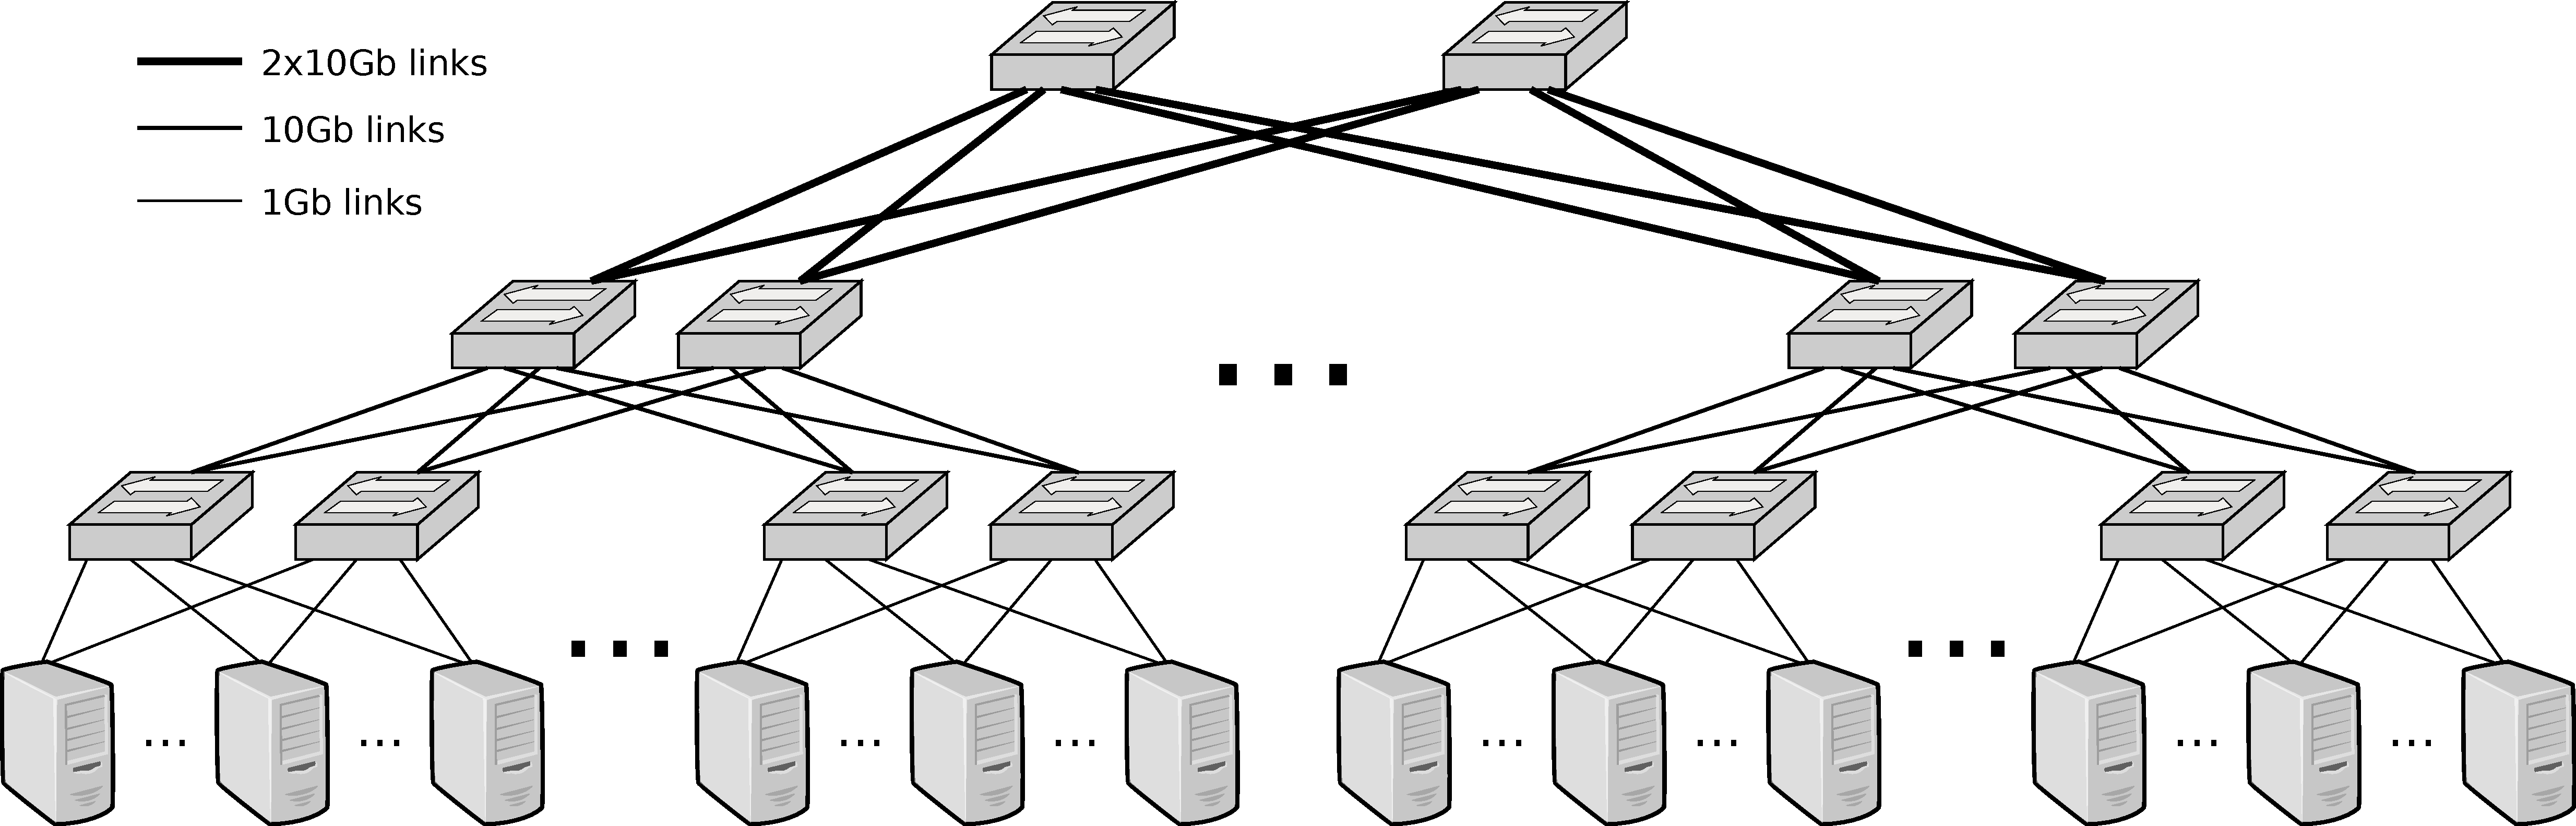
\includegraphics[width=\textwidth]{img/fat_tree}
\caption{A fat-tree network topology with redundant links for fault tolerance}\label{fig: fat tree}
\end{figure}


\subsubsection{Storage}

SAN, or local disk

One or multiple DFS, available to part of the infrastructure
\subsubsection{From server housing to container housing}

A recent trend in datacenter design relies on the usage of shipping containers to embed the servers~\cite{containers}. In practice, a container can be considered as a datacenter. It may embeds
thousands of servers with their network~\cite{guo2009bcube}, their storage and their cooling systems.
Shipping containers of servers are then currently used as a building block for  large scale datacenters.
Containers are first very energy-efficient while they allow to expand the hosting capacity of a datacenter easily by acquiring and plugin new containers when needed.


Hosting platforms: clouds (amazon~\cite{amazon}, rackspace~\cite{rackspace}, azure~\cite{azure}), testbeds such as Emulab~\cite{emulab} or Grid'5000~\cite{g5k}.

\subsection{Virtualized applications}

User want to have its application running into the platform

Either instantiate an existing template that is already customized for the hosting
platform. As an example Amazon  EC2 has a list of pre-made instances

otherwise, create from scratch.
Justify replication: elastic computing, absord load

Figure~\ref{fig: 3tiers} illustrates a typical 3-tier HA Web application.
The first tier is composed of 3 VMs, each running one Apache HTTP server~\cite{apache-http}.
The second tier is made up with 2 VMs, each running one Apache Tomcat instance~\cite{apache-tomcat}.
The third tier is made up with 2 VMs, each running one instance of the MySQL database~\cite{mysql}.
Each instance of Apache HTTP and Apache Tomcat includes a load balancer to spread out the requests
associated to servlets or the database respectively.

The Apache services in tier 1 and the Tomcat services in tier 2
are stateless: all the handled requests are independent transactions
and no synchronization of their state is required. On the other hand,
tier 3 runs a replicated MySQL database, which is stateful:
transactions that modify the data must be propagated from one VM
hosting a replica of tier 3 to the others, to maintain a globally
consistent state.
%
In this setting, the application administrator has three expectations.
First, the VMs must be running on servers having enough resources to make the services
work at peak level.
Second, the VM replicas must be running on distinct servers to provide the awaited
fault tolerance to hardware failure.
Finally, the VMs in the Tiers 3 must be running on servers connected by a low latency
medium that reduce the overhead of the databases synchronization protocol.


\begin{figure}[htb]
\centering
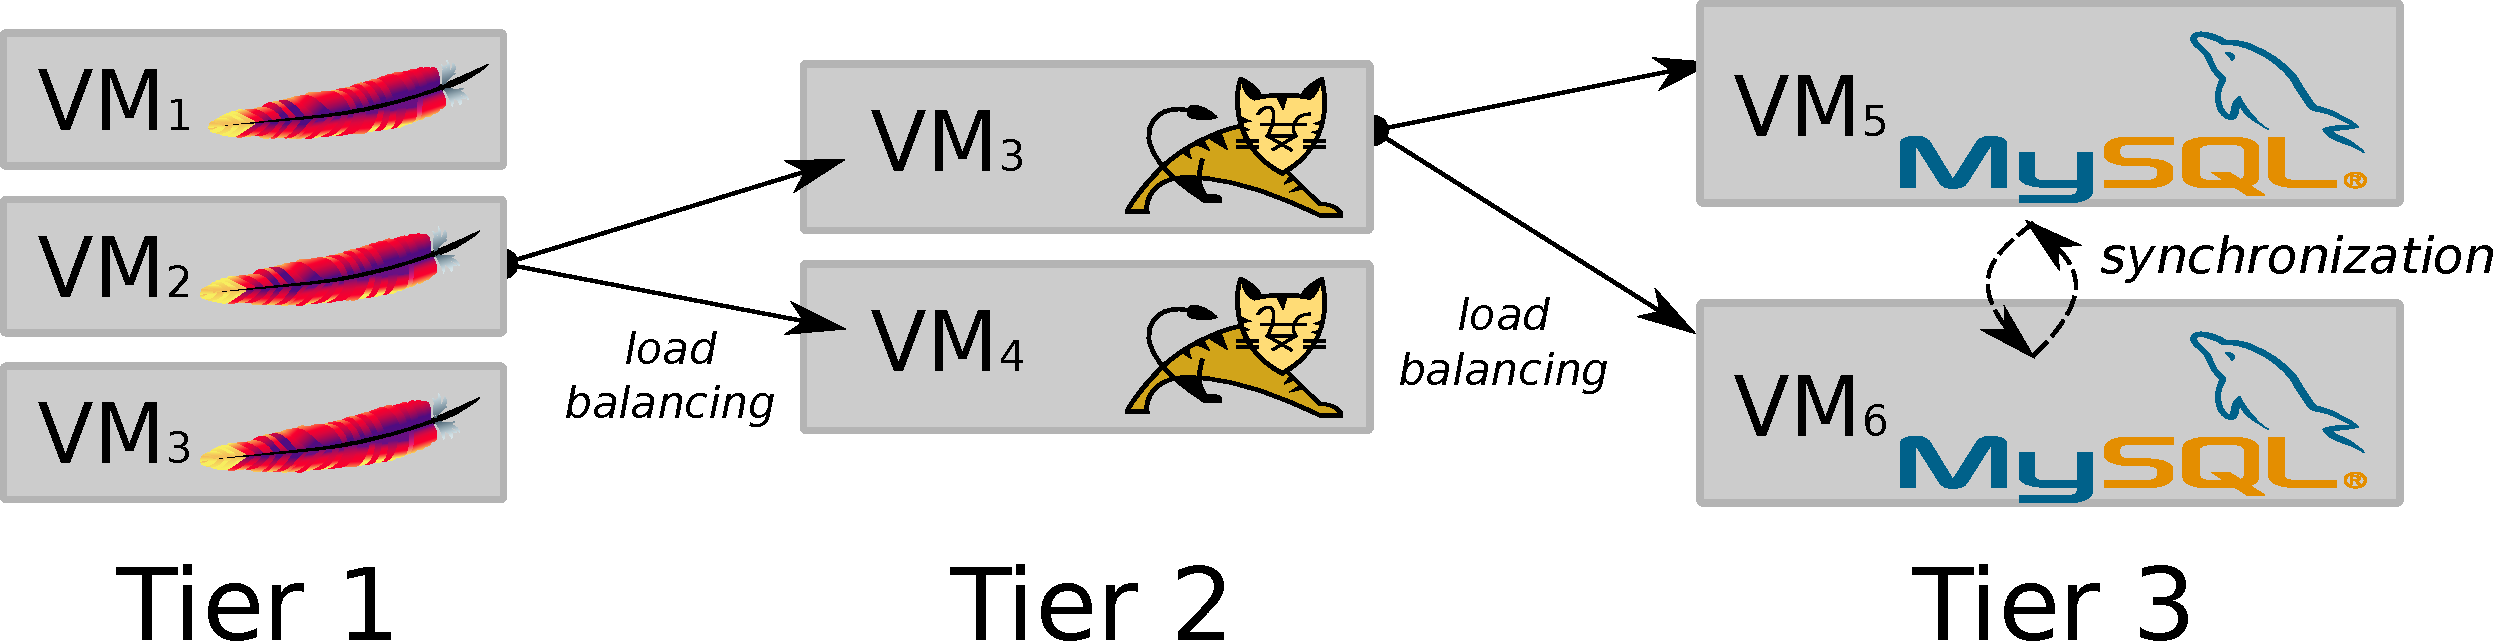
\includegraphics[width=.8\textwidth]{img/3tiers}
\caption{Sample architecture for a Highly-Available web service.}\label{fig: 3tiers}
\end{figure}

\section{Hosting platform management}

\subsection{VM management}

Through its lifetime on the platform, the state of a virtual machine is subject to change during a
reconfiguration process. Figure~\ref{fig:  vm lifecycle} depicts as a finite state automaton the six
possible states for a virtual machines and the action to apply to perform the transition between one
state to another. 


\begin{figure}[htb]
\centering
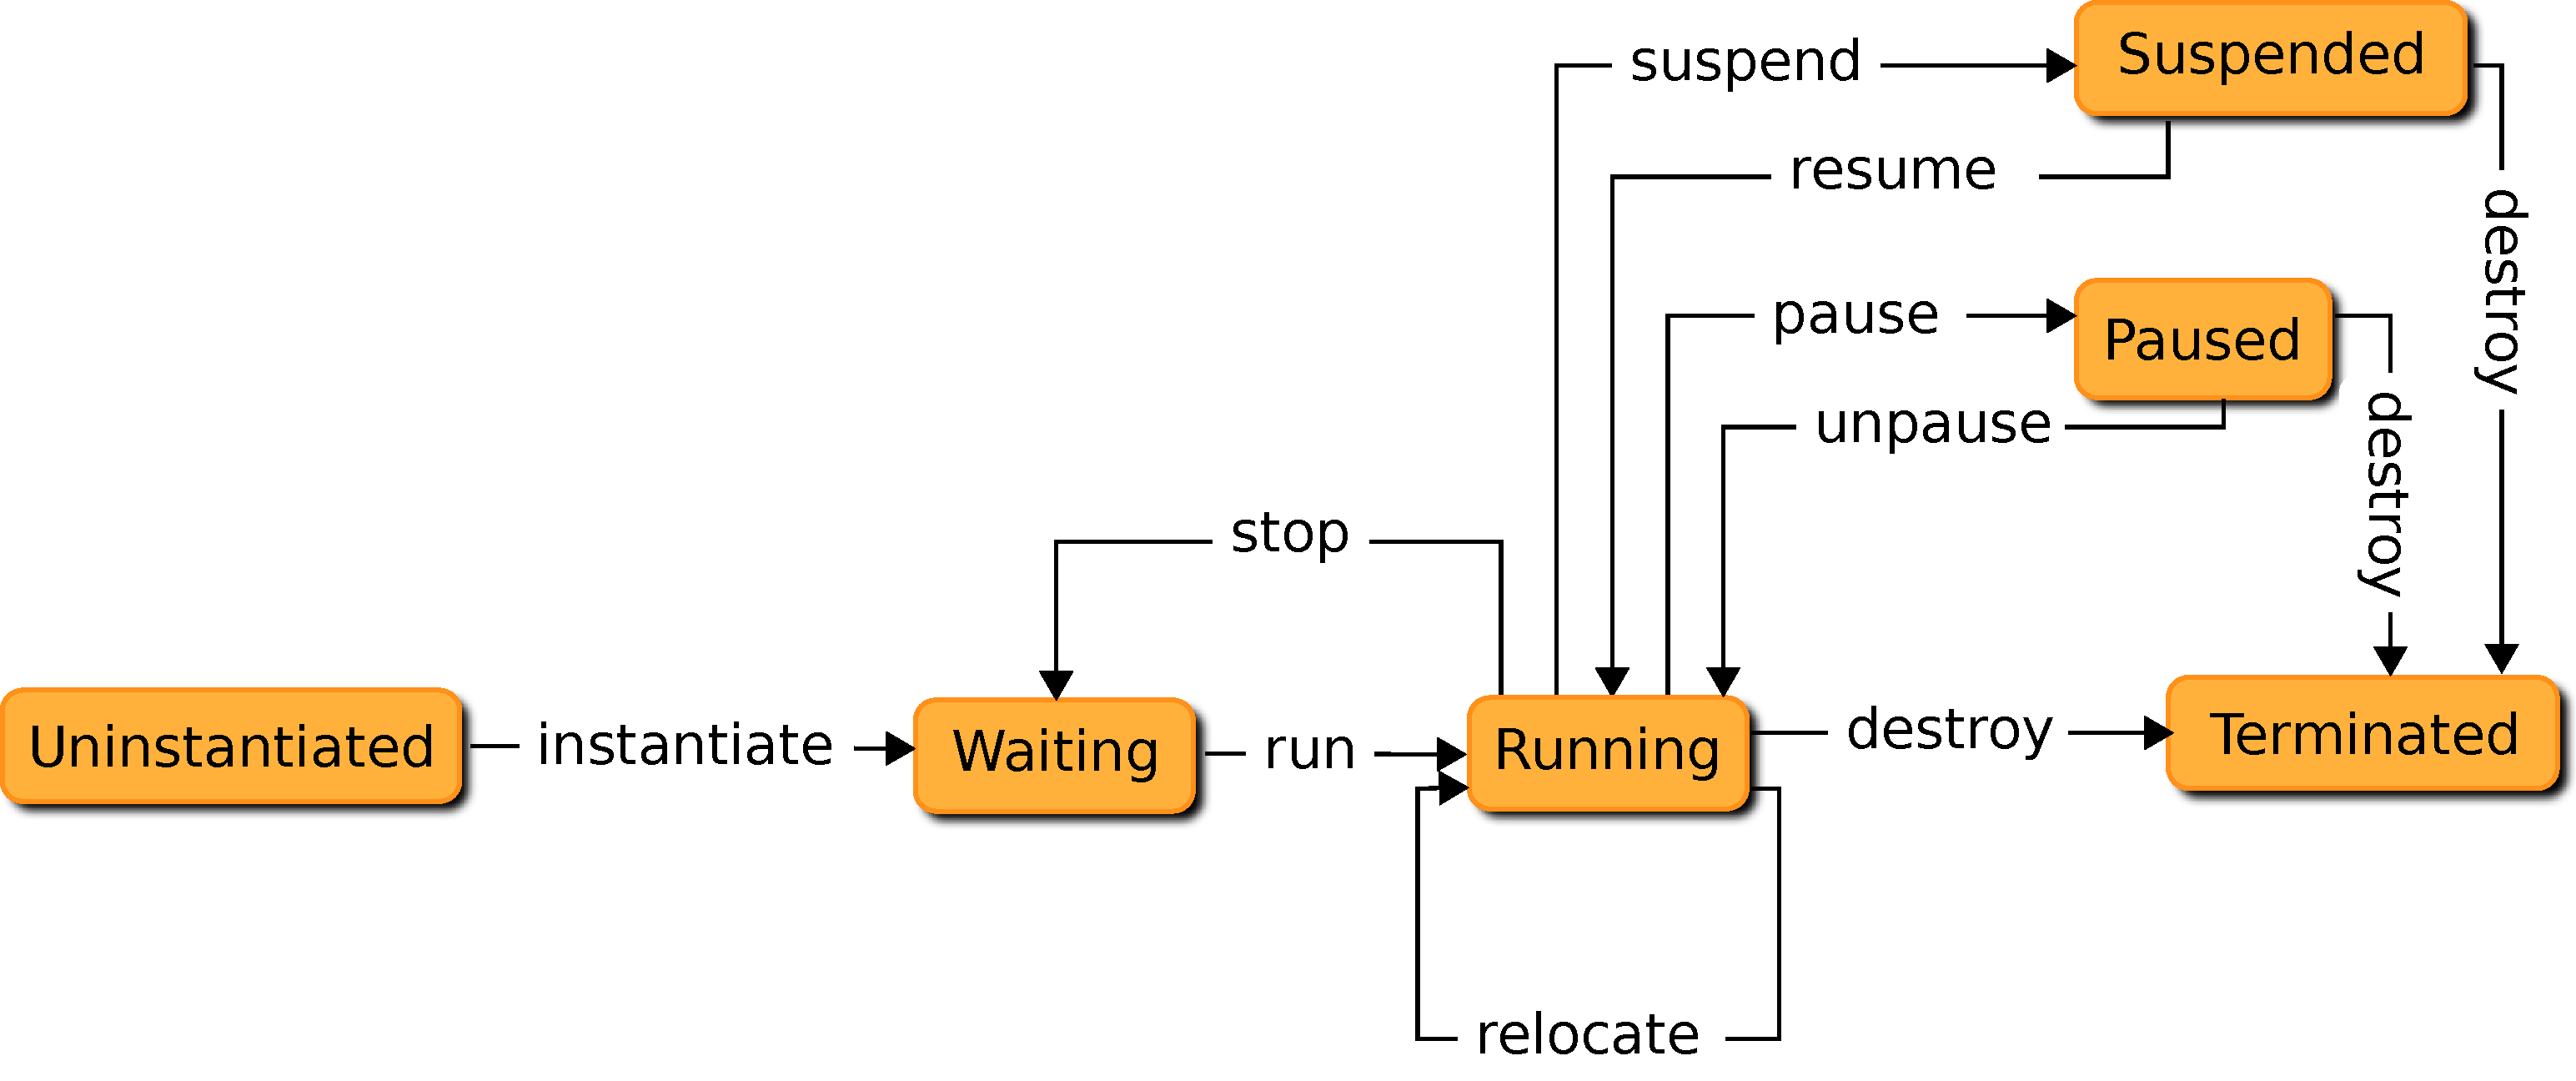
\includegraphics[width=\textwidth]{img/VM_lifecycle}
\caption{Lifecycle of a virtual machine}\label{fig: vm lifecycle}
\end{figure}


\subsubsection{Uninstantiated}
The \st{Uninstantiated} state is the initial state for any virtual machine. At this stage, the virtual machine is not prepared to be deployed on the servers.
The action \emph{instantiate} leads to prepare the virtual machine for the hosting platforms. This may imply several platform dependent operations such as the creation of configuration files to describe the virtual machine, but also the preparation of its disk image from a template or from scratch.
At the end of the \emph{instantiate} action, the virtual machine lies in the \st{Waiting} state.


\subsubsection{Waiting}
The \st{Waiting} state denotes a virtual machine that has been configured to be deployed on a server.
The action \emph{run} will then deploy the virtual machine on a given server. The virtual machine will be booted and will start to consume resources. The action is not necessarily synchronous and may immediately end once the booting process of the virtual machine is engaged despite it is not available to its owner.
At the end of the action, the virtual machine lies in the \st{Running} state.

\subsubsection{Running}
The \st{Running} state denotes a virtual machine that is running on a server. Several actions are then
possible to manipulate the state or the location of the virtual machine.

The \emph{relocate} action is responsible of relocating of the virtual machine to another server.
Such an action can be achieved in different manners, depending on the hypervisors capabilities, the virtual machine specification and the software it embeds.
%
Live migration~\cite{clark-nsdi2005,vmotion} is the most known technique to relocate a running virtual machine. It consists in moving the virtual machine to a given server with a negligible downtime. In practice, the virtual machine configuration, context and memory are copied in background to an inactive virtual machine
on the destination server. Once the state of the running virtual machine is mostly coherent with the state of the inactive virtual machine on the destination server, the running virtual machine is suspended to finalize the transfer and the virtual machine on the destination server is activated. The original virtual machine is finally destroyed.
%
\emph{Cold} migration is another solution where the virtual machine on the source server is set inactive before performing the transfer. 
%
Finally, if the virtual machine hosts a replicated service, it is also possible to simply instantiate a new virtual machine on the destination server then stop the original virtual machine once the new one is booted.
Such an operation is however more intrusive as it implies to know the embedded softwares.

The \emph{pause} action blocks the virtual CPUs allocated to the virtual machine. At the end of this action, the virtual machine lies in the \st{Paused} state.

The \emph{suspend} action suspends the virtual machine on a disk. The virtual CPUs allocated to the virtual machine are paused and its memory is copied on the disk. At the end of this action, the virtual machine lies in the \st{Suspended} state.

The \emph{stop} action shutdown a virtual machine gracefully in a similar way a computer is turned off. At the end of the action, the virtual machine is back into the \st{Waiting} state and is supposed to be re-used.

\subsubsection{Paused}
The \st{Paused} state indicates the virtual machine is suspended into the server memory. The virtual machine memory is still lying on its hosting server memory but its virtual CPUs have been blocked. The virtual machine is then not available to its administrator. The \emph{unpause} action moves the virtual machine back into the \st{Running} state by unblocking its virtual CPUs.

\subsubsection{Suspended}
The \st{Suspended} state indicates the virtual machine is suspended into a disk. A consistent image
of the VM memory and state has been stored on a disk. The virtual machine no longer consumes any physical resources except disk storage. The \emph{resume} action moves the virtual machine back into the \st{Running} state by restoring its memory and its state from the disk image.

\subsubsection{Terminated}
\smallskip
The \emph{destroy} action can be used from the states \st{Running}, \st{Suspended}, or \st{Paused} to set a virtual machine in the \st{Terminated} state. The action brutally stops the virtual machine. This corresponds to a hard shutdown on a computer when it is powered off instantly. As the virtual machine has been stopped brutally, its disk image may be corrupted. It is then not sure the virtual machine can be restarted.
We then consider the \st{Terminated} state as a terminal state.


\subsection{Server management}

Similar to a virtual machine, a hosting server also has its state updated through actions during its lifecycle. Figure~\ref{fig: server lifecycle} depicts as a finite state automaton, the two possible states for a server
and the action to apply to perform the transition between one state to another.

\begin{figure}[htb]
\centering
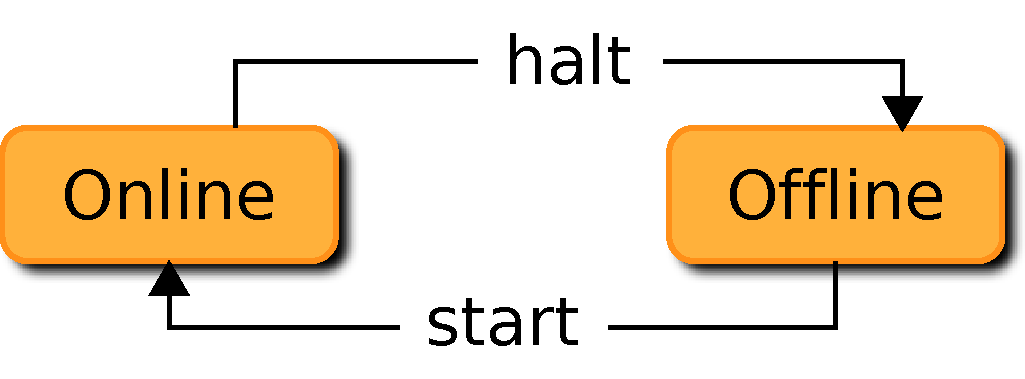
\includegraphics[width=4.4cm]{img/server_lifecycle}
\caption{Lifecycle of a server}\label{fig: server lifecycle}
\end{figure}

\subsubsection{Online}
The \st{Online} state indicates the server is available to the hosting platform and may host virtual machines. The \emph{halt} action is responsible of setting the server in the \st{Offline} state.

\subsubsection{Offline}
The \st{Offline} state indicates the server is not directly available to the hosting platforms. It can be made available using the action \emph{start}. The \st{Offline} state can be provided using different approaches. The traditional approach is to turn the server off. The action \emph{start} will then boot it.
It may also be convenient to suspend the server into disk or into RAM. Such a physical state has the same properties with regards to the external users as it is not directly available to them. However, restoring a server from a suspend-to-RAM or suspend-to-disk state may provide a faster response time with regards to a traditional unpowered state.

\section{Reconfiguration}

Occurs when actions have to be executed. Typically motivated by the arrival, departure of VMs, 
server maintenance or SLA violation fix or overal usage improvement.


%History

% from datacenter to hosting platform



% Hosting platforms

%% infrastructure

% - Interconnected servers
% - racks


% - SAN or local disk for storage

%% Virtualization


%History
%Datacenters
% Storage: SAN or local disk, pure image or cow,

% Hosting platforms
% Infrastructure

%Virtualization

%cluster on demand


% reconfiguration


A reconfiguration occurs when the current platform configuration does not meet the tenants or the platform
administrator expectations. During a reconfiguration, several management operations
are performed to put back the hosting platform into a viable configuration. These operations
typically manipulate the virtual machines' state or placement, their resource allocation, or the servers' state.

In this chapter, we describe the principles of a reconfiguration process.
In a first Section, we describe the management actions that can be performed during a reconfiguration and
their impact on the servers and the virtual machines.
In a second Section, we discuss about the necessity of scheduling the action execution to ensure
the reliability of the reconfiguration process. 
Finally, we present a sample reconfiguration.

The action to execute during a reconfiguration process manipulate the virtual machines and the servers' states and the allocation of the servers resources.

First, any action on a virtual machine is exclusive as it impacts either it state or its location. In this setting, to operate on a virtual machine, the virtual machine must be in a state and no actions must already be pending. In addition, performing an action on a virtual machine alter the resource offered by its hosting server in two ways. In practice, an action may liberate or consume some resources on the hosting server. Table~\ref{tab: vm impact resources} details this impact per action.

\begin{table}[htdp]
\centering
\begin{tabular}{l |  c  c }
Action 		& Liberating  & Consuming \\\hline\hline
instantiate		&  		     &		        \\
run			& 		     & \checked	\\
relocate		& \checked   & \checked	\\
destroy		& \checked   & \\
suspend		& \checked   & \\
resume		& 		    & \checked \\
pause		& \checked   &	\\
unpause		& 		    & \checked 
\end{tabular}
\caption{Impact on actions related to a virtual machine on its hosting server}\label{tab: vm impact resources}
\end{table}

The \emph{run} and the \emph{resume} actions are similar in terms of resource occupation. Indeed, in both situations, the manipulated virtual machine was not consuming any resources and once the action started, the virtual machine starts consuming resources on its hosting server.
The \emph{suspend}, the \emph{stop}, and the \emph{destroy} actions are also similar. Indeed, the manipulated virtual machine was running on the server. Once the action executed, the virtual machine is no longer running and all the allocated resources are freed.
The \emph{pause} action liberates only a part of the resources allocated to the manipulated virtual machine. In practice, every resources except the memory are liberated. The \emph{unease} action
makes then the virtual machine consumes all other resources again.
Finally, the \emph{relocate} action is both an action that liberate and consume resources. Indeed, once the action executed, the virtual machine is running on another server. In this situation, the resources that was consumed on the origin server were liberated while the virtual machine consumes now resources on its new host.

Actions related on the management of a server also impacts the resources available to the virtual machine. Table~\ref{tab: server impact resources} details this impact for every action.
The \emph{start} actions makes the server online and potentially available to host virtual machine. This action liberates then the resources that was busy due to the non-availability of the server. On the opposite, the action \emph{halt} makes the server offline so, consumes every resources on the server.

\begin{table}[htdp]
\centering
\begin{tabular}{l |  c  c }
Action 		& Liberating  & Consuming \\\hline\hline
start			&  \checked   &		        \\
halt			& 		     & \checked	\\
\end{tabular}
\caption{Impact on actions related to a virtual machine on its hosting server}\label{tab: server impact resources}
\end{table}

Consuming actions have then preconditions to be executed. These preconditions consists in having enough free resource on the target server to perform the action. Typically, enough memory, CPU, disk space, \etc. 
%
Aside, actions on virtual machines and servers are closely related as action related on a virtual machine hosted on a server requires to have the involved servers online. While turning off a server requires to have this server not hosting any virtual machine.

As a result, actions may have to be planned depending on their resource profile. Scheduling the 
So, in addition to the state of the virtual machines, the servers,  the placement of the virtual machines on the servers, and the resource allocation, the temporality of the actions must be considered to ensure the reliability of the reconfiguration process.

\section{A sample reconfiguration}

Let's consider a hosting platform of 4 servers (N1 to N4) managing a total of 6 virtual machines (VM1 to VM6). Figure~\ref{fig: sample reconfiguration} depicts an initial and a destination configuration
to reach. Initially, virtual machines VM1 and VM2 are in the \st{running} state on the server N1. The virtual machines VM3, VM5, and VM6 are in the \st{Running} station servers N2, N3, and N4, respectively. Finally, the virtual machine VM4 is in the \st{Waiting} state. In we consider that 1) every virtual machine must have an access to enough uCPU and memory capacity, 2) VM4 must be in the \st{Running} state, and 3) N3 must be in the \st{Offline} state, then this configuration is not viable.


\begin{figure}[htb]
\centering
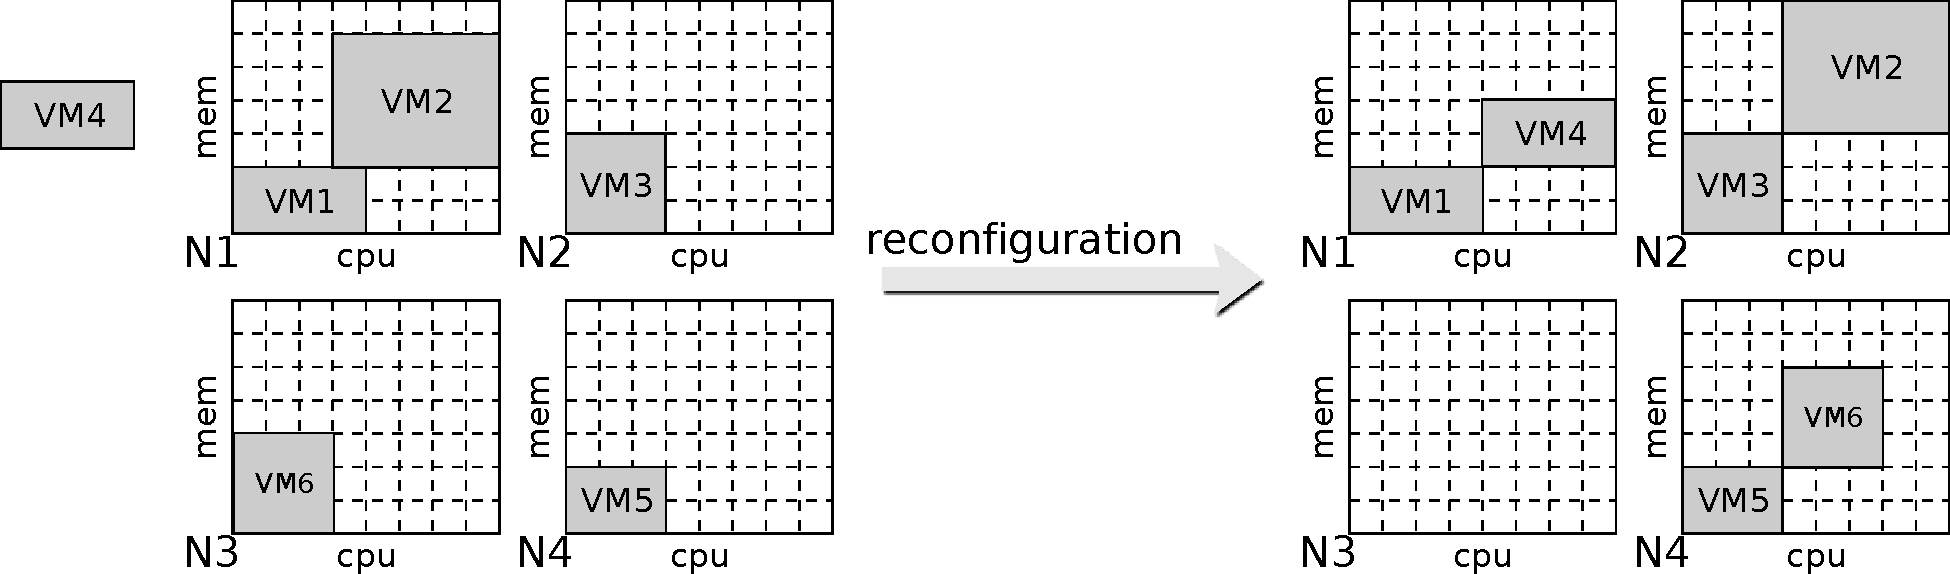
\includegraphics[width=\textwidth]{img/sample_reconfiguration2}
\caption{A reconfiguration between a non-viable configuration and a destination configuration}\label{fig: sample reconfiguration}
\end{figure}


The destination configuration pictured on the right satisfies every prerequisite. One possible reconfiguration process to achieve the transition between the source and the destination configuration
consists to execute 4 actions. N3 has to be halted, VM4 must run on N1, VM2 and VM6 must be relocated to N2 and N4 respectively. 
%
However, it is not possible to execute these actions in any order. As an example, it is not possible to
execute the \emph{halt} action on N3 until VM6 is away or to run VM4 on N1 before relocating VM4 to N2 as their is no enough free resources at this point.
%
Figure~\ref{fig: eo sample reconfiguration}. depicts a possible event-oriented reconfiguration plan to ensure the termination of every actions. At startup, it is possible to relocate VM2 and VM6 in parallel. Once VM6 is running on N4, then it is possible to halt N3. Finally, once VM2 is running on N2, then VM4 can be deployed on N1.



\begin{reconfPlan}
\centering
\begin{tabular}{ll}
\O & $\rightarrow$ relocate(VM2) \& relocate(VM6)\\
!relocate(VM6) &$\rightarrow$ halt(N3)\\
!relocate(VM2)\ & $\rightarrow$ run(VM4)
\end{tabular}
\caption{Event-based reconfiguration plan that ensure the termination of the reconfiguration process
depicted in Figure~\ref{fig: sample reconfiguration}.}\label{fig: eo sample reconfiguration}
\end{reconfPlan}


Another solution to express sequences of actions in a reconfiguration plan consists in providing
a theoretical duration for each each then computing a actions schedule. 
Table~\ref{tab: actions duration} shows an estimated duration for each action composing
the reconfiguration process in Figure~\ref{fig: sample reconfiguration}. 
Table~\ref{tab: tb sample reconfiguration} depicts then a timer-based reconfiguration plan.
\todo{From a theoretical timer-based rp to a reliable practical one.}

\begin{table}[htb]
\centering
\begin{tabular}{l | c}
relocate(VM2) & 0'02 \\
relocate(VM6) & 0'06 \\
run(VM4) & 0'06 \\
halt(N3) & 0'06
\end{tabular}
\caption{Estimated actions duration}
\label{tab: actions duration}
\end{table}


\begin{table}[htb]
\centering
%\small
\begin{tabular}{ c | c || l }
Start & End & Action \\\hline
0'00 & 0'02 & relocate(VM2) \\
0'00 & 0'05 & relocate(VM6) \\ 
0'02 & 0'08 & run(VM4)\\
0'05 & 0'11 & halt(N3) \\
\end{tabular}

\caption{Timer-based reconfiguration plan that ensure the termination of the reconfiguration process depicted in Figure~\ref{fig: sample reconfiguration}.}\label{tab: tb sample reconfiguration}

\label{tab: tb sample duration}
\end{table}

\section{Conclusion}

Reconfiguration process, act on the state of the virtual machine, its resource allocation, and its placement. Also acts on the servers state.

Several actions, to be feasible, have preconditions related to the state of the manipulated and the involved elements but also preconditions related to the available resources on the server.

The model describing a customizable reconfiguration problem must then provides these bases to be able to be customized enough. In the next chapter, we then present a mathematical model to specify
a reconfiguration process.

Principles

Next:
A formal model to represent a reconfiguration
late amount of constraints, leaded by technology innovation, application type, platform capabilities, trends


